\addcontentsline{toc}{chapter}{LAMPIRAN}
\titleformat{\section}{\normalfont\bfseries}{\thesection}{1em}{}
% Format judul untuk bagian lampiran
\chapter*{LAMPIRAN}

%\thispagestyle{plain} % Halaman pertama bab menggunakan gaya plain
\newappendix{LAMPIRAN 1. DATA KUESIONER PETANI}
\begin{figure}[H]
    \centering
    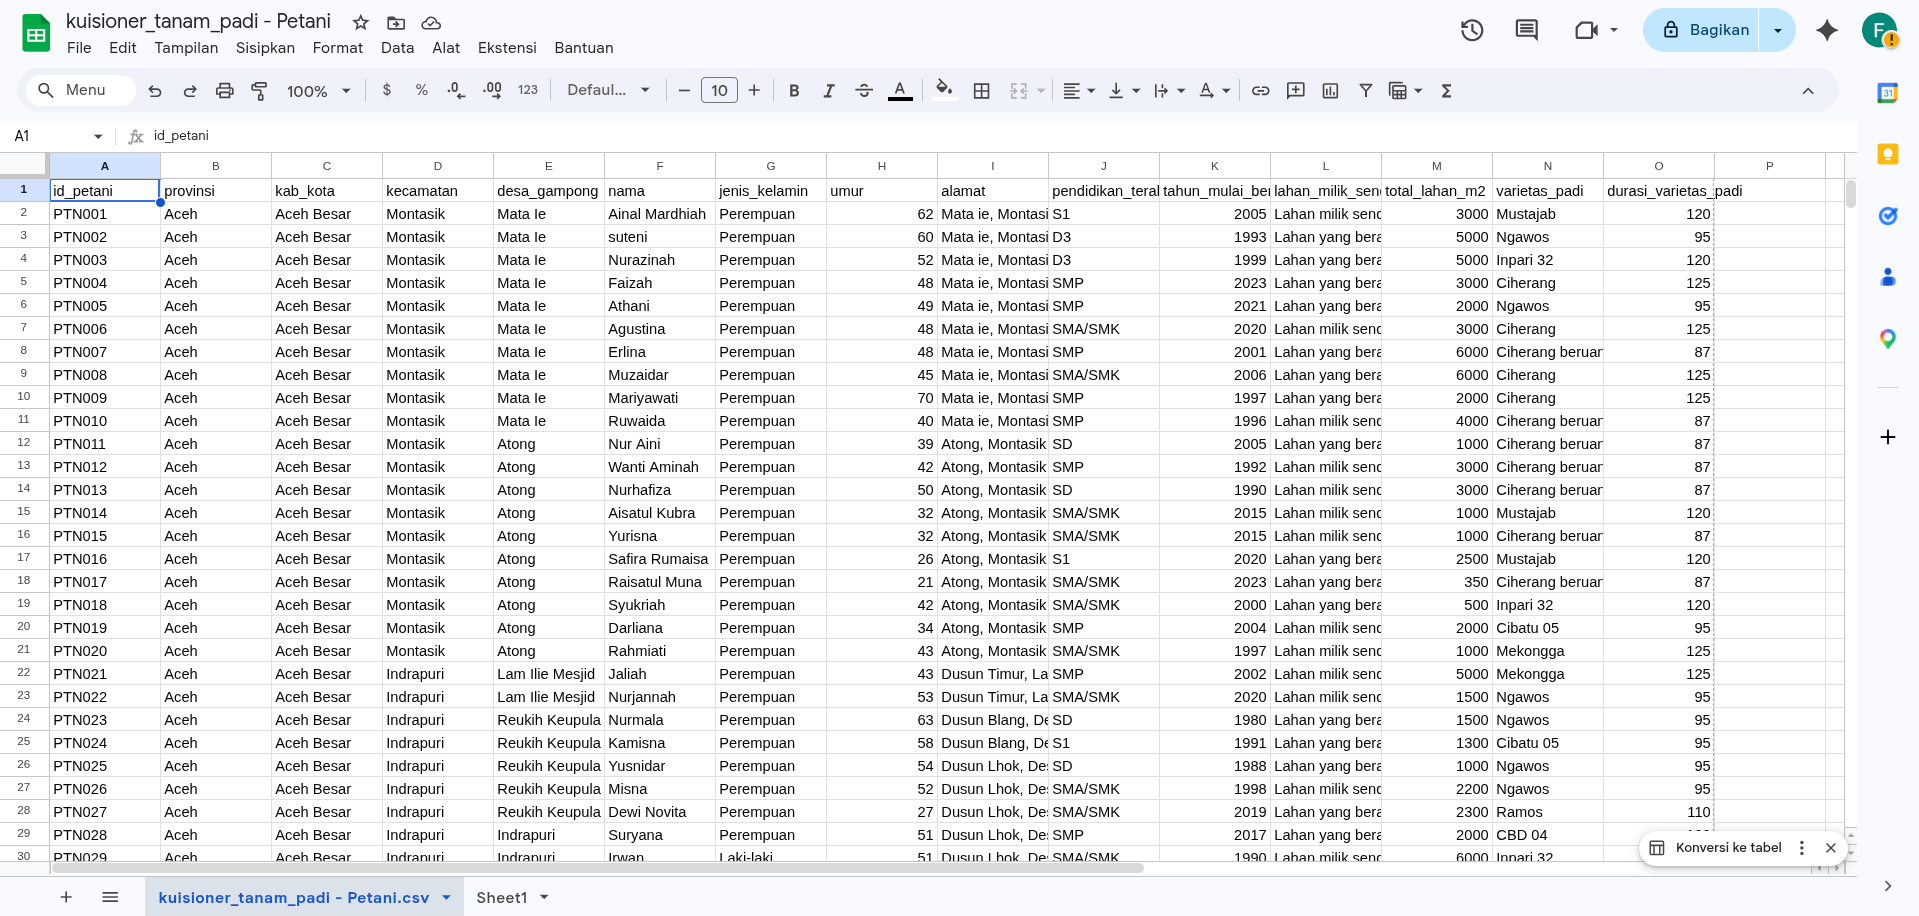
\includegraphics[width=\linewidth]{image/lampiran/1_kuisioner.png}
    \caption{Kuesioner petani di Kabupaten Aceh Besar}
    \label{lamp:kuisioner}
\end{figure}

\newappendix{LAMPIRAN 2. DATA PENELITIAN}
\begin{figure}[H]
    \centering
    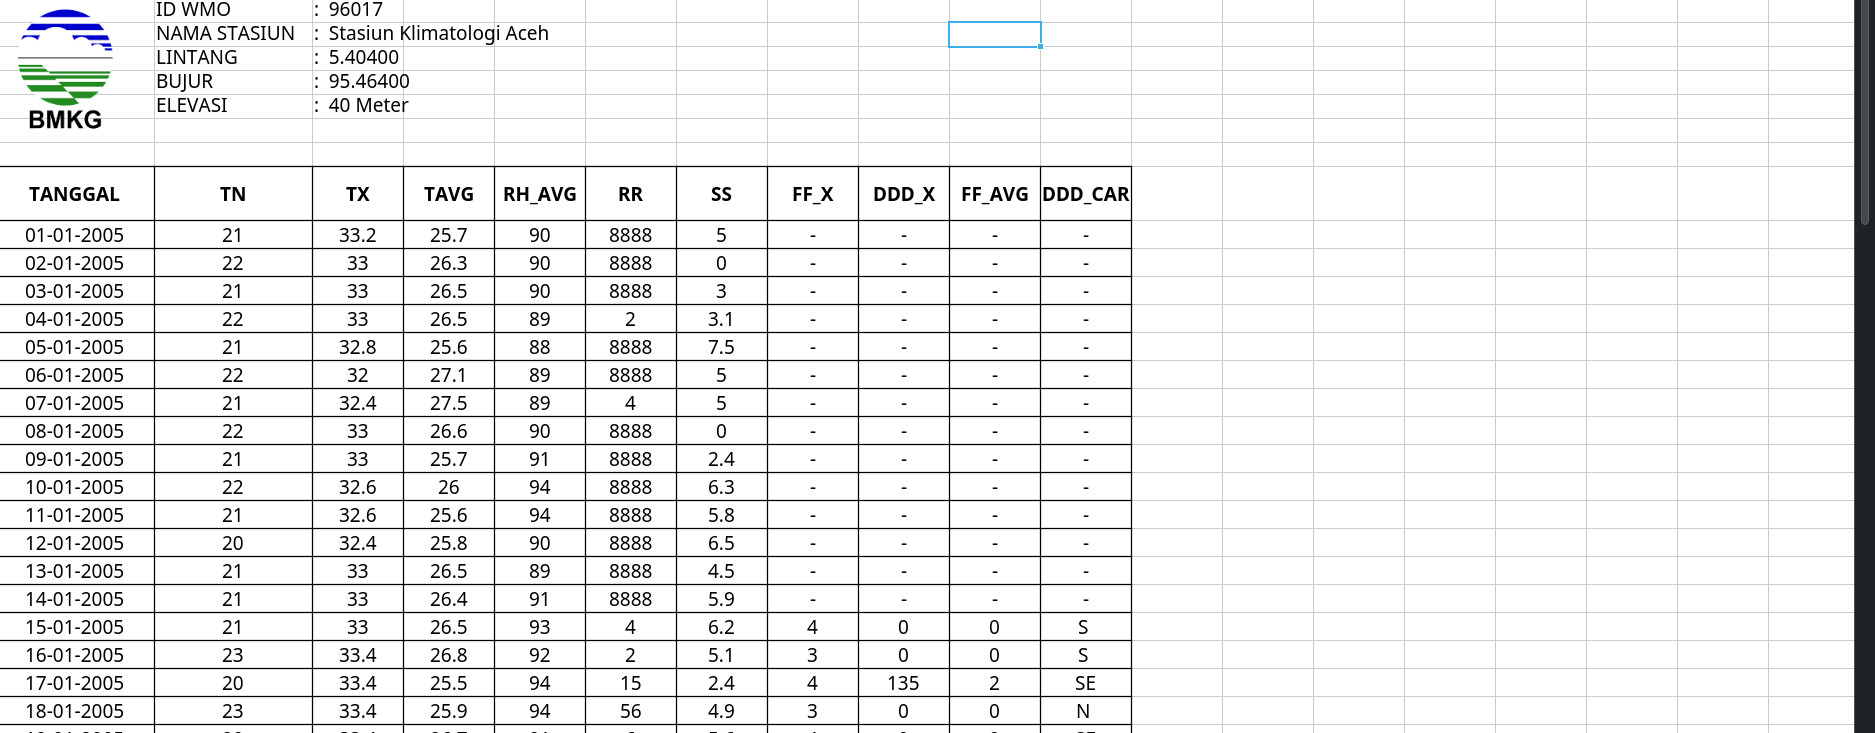
\includegraphics[width=\linewidth]{image/lampiran/2_data_penelitian_bmkg.png}
    \caption{Data penelitian BMKG}
    \label{lamp:data_penelitian_bmkg}
\end{figure}
\begin{figure}[H]
    \centering
    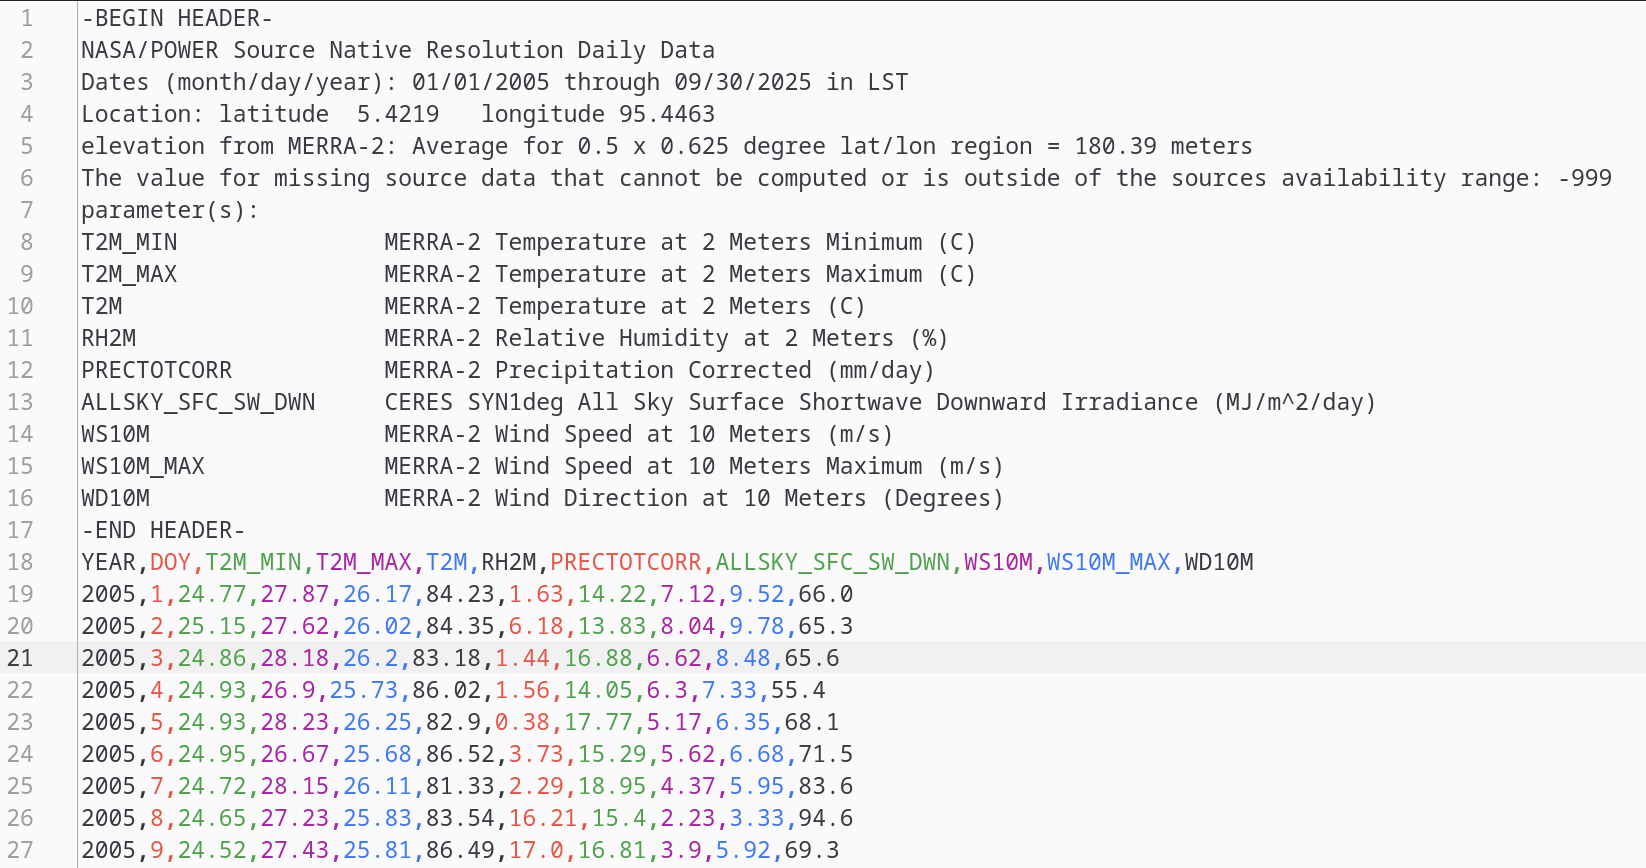
\includegraphics[width=\linewidth]{image/lampiran/2_data_penelitian_nasa.png}
    \caption{Data penelitian NASA POWER}
    \label{lamp:data_penelitian_nasa}
\end{figure}

\newappendix{LAMPIRAN 3. BUKTI PENGERJAAN SPRINT}
\begin{figure}[H]
    \centering
    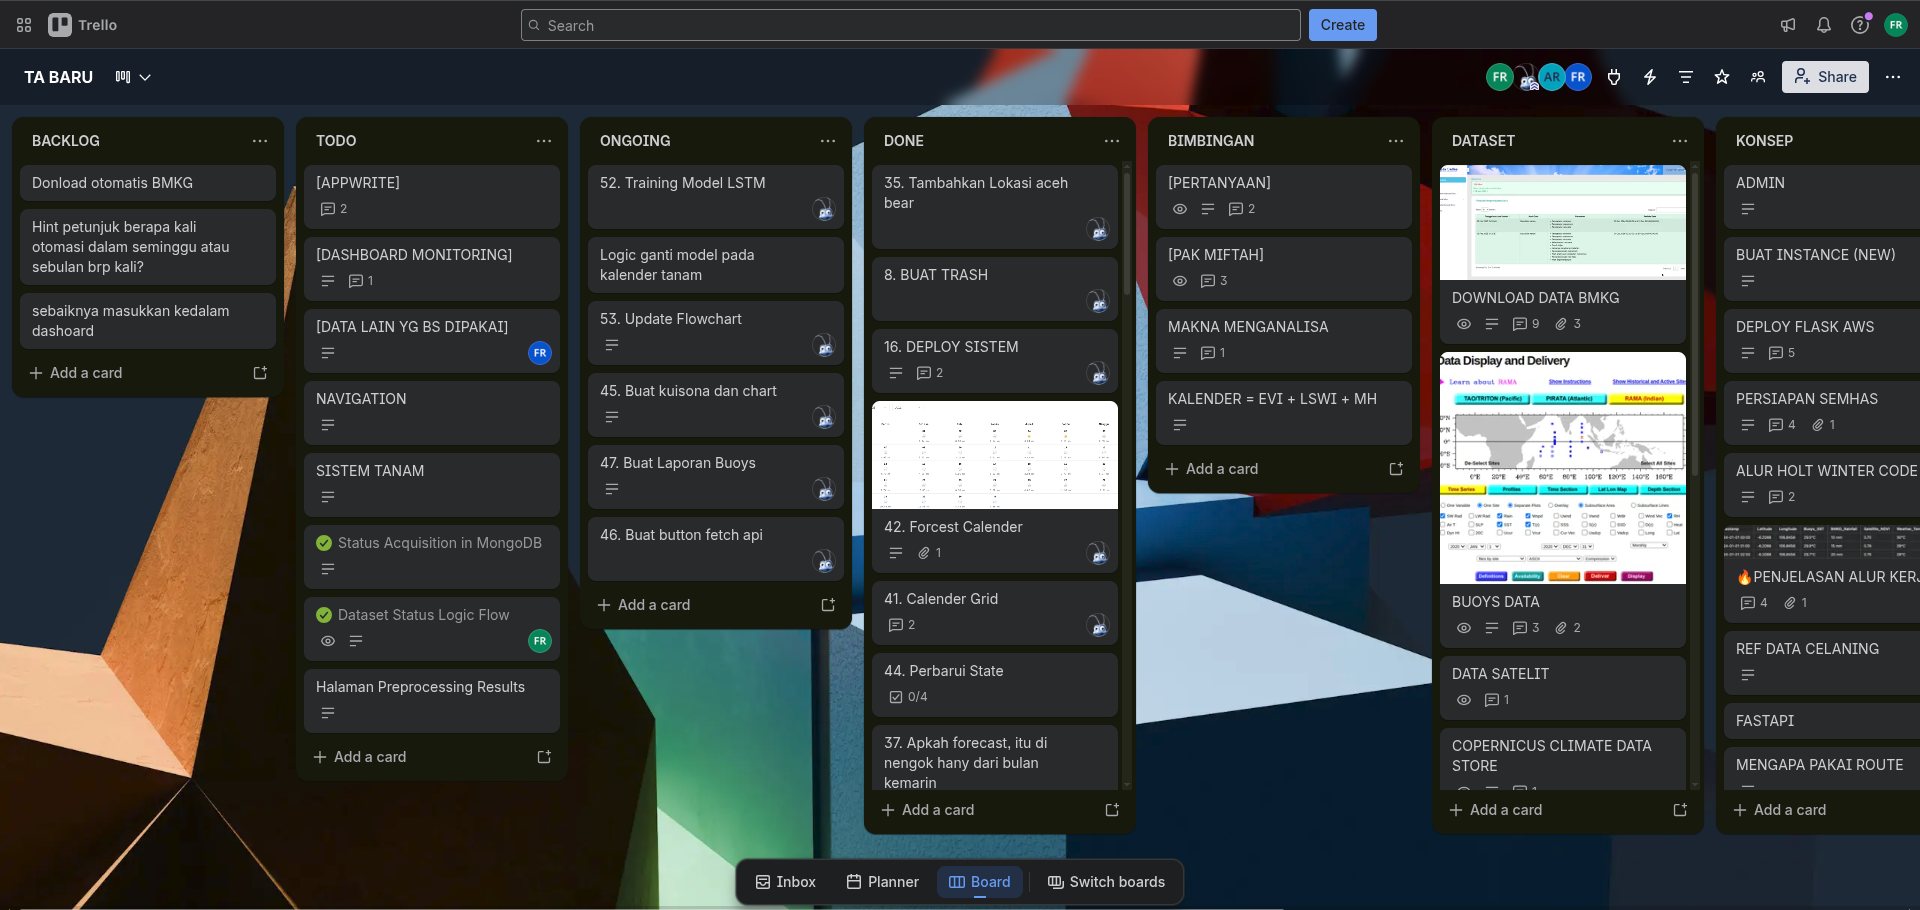
\includegraphics[width=\linewidth]{image/lampiran/3_sprint.png}
    \caption{Dokumentasi pengerjaan sprint pengembangan sistem}
    \label{lamp:sprint}
\end{figure}

\newappendix{LAMPIRAN 4. IMPLEMENTASI DATABASE MONGODB}
\begin{figure}[H]
    \centering
    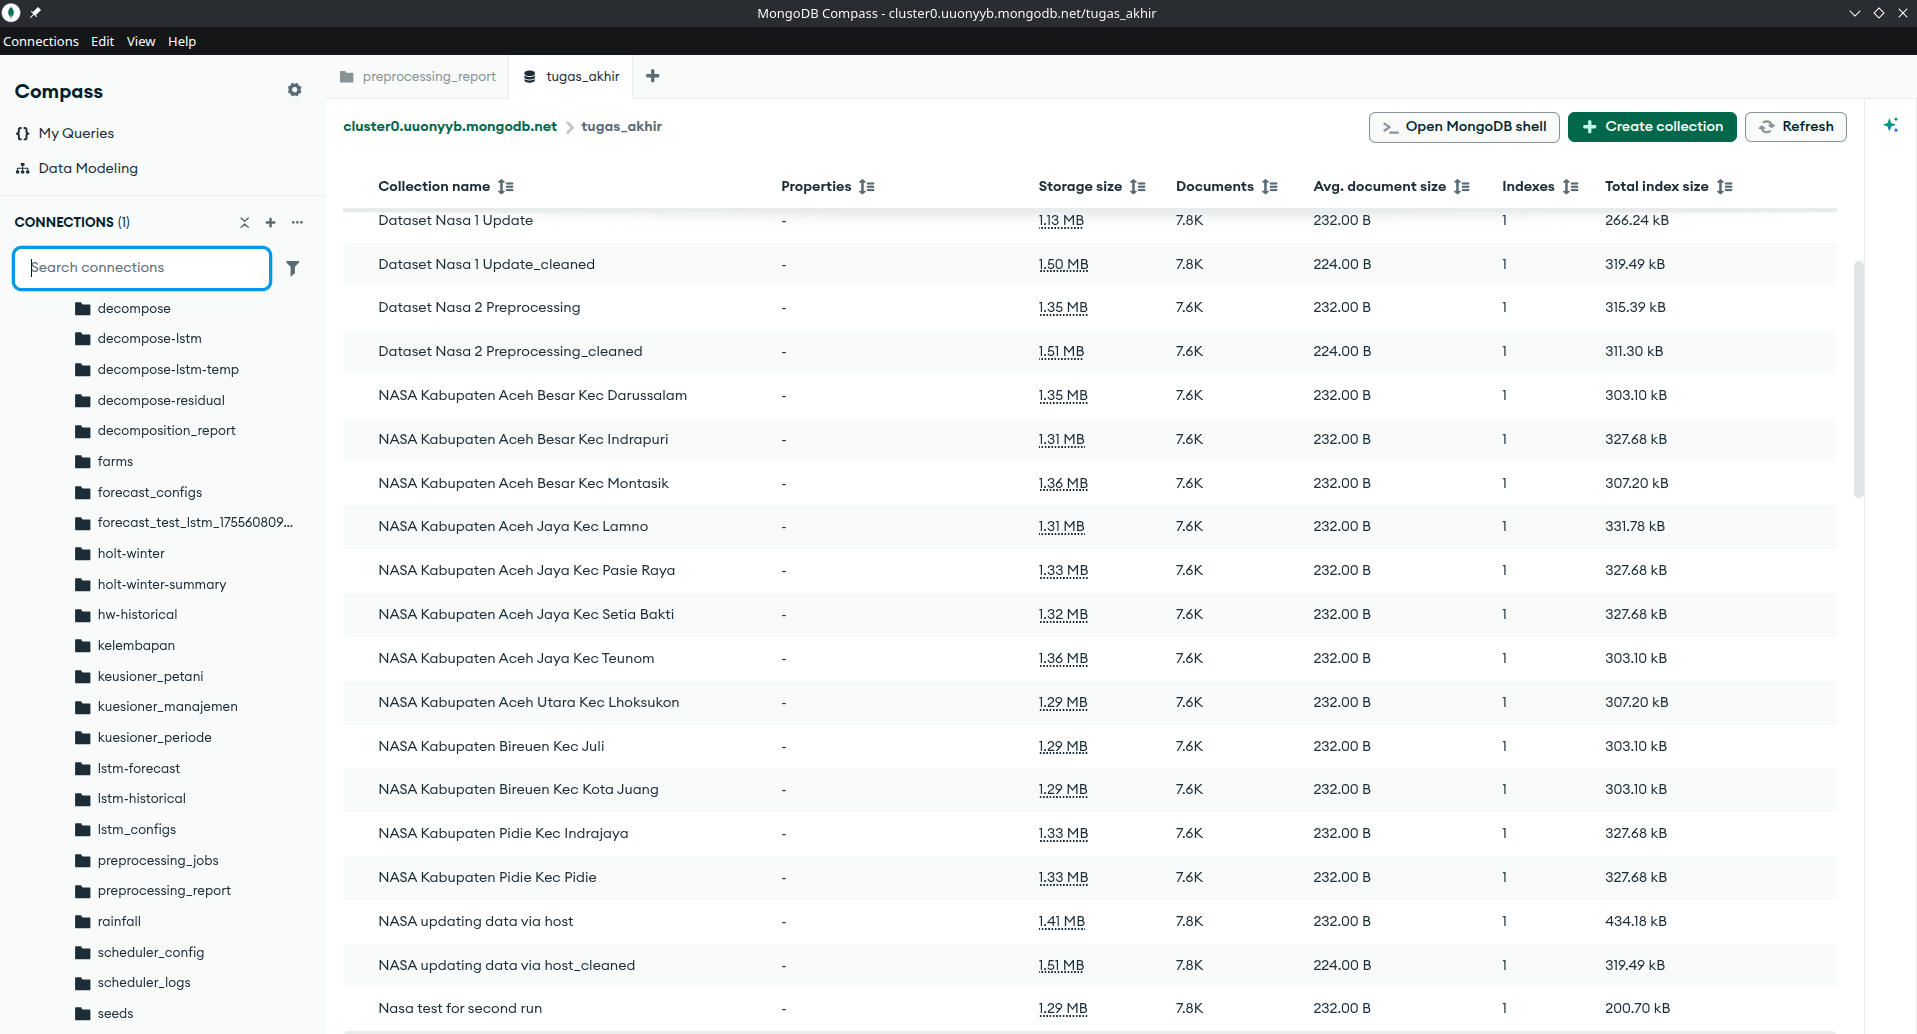
\includegraphics[width=\linewidth]{image/lampiran/4_databse.png}
    \caption{Implementasi skema database MongoDB}
    \label{lamp:database}
\end{figure}

\newappendix{LAMPIRAN 5. PENGUJIAN API MENGGUNAKAN POSTMAN}
\begin{figure}[H]
    \centering
    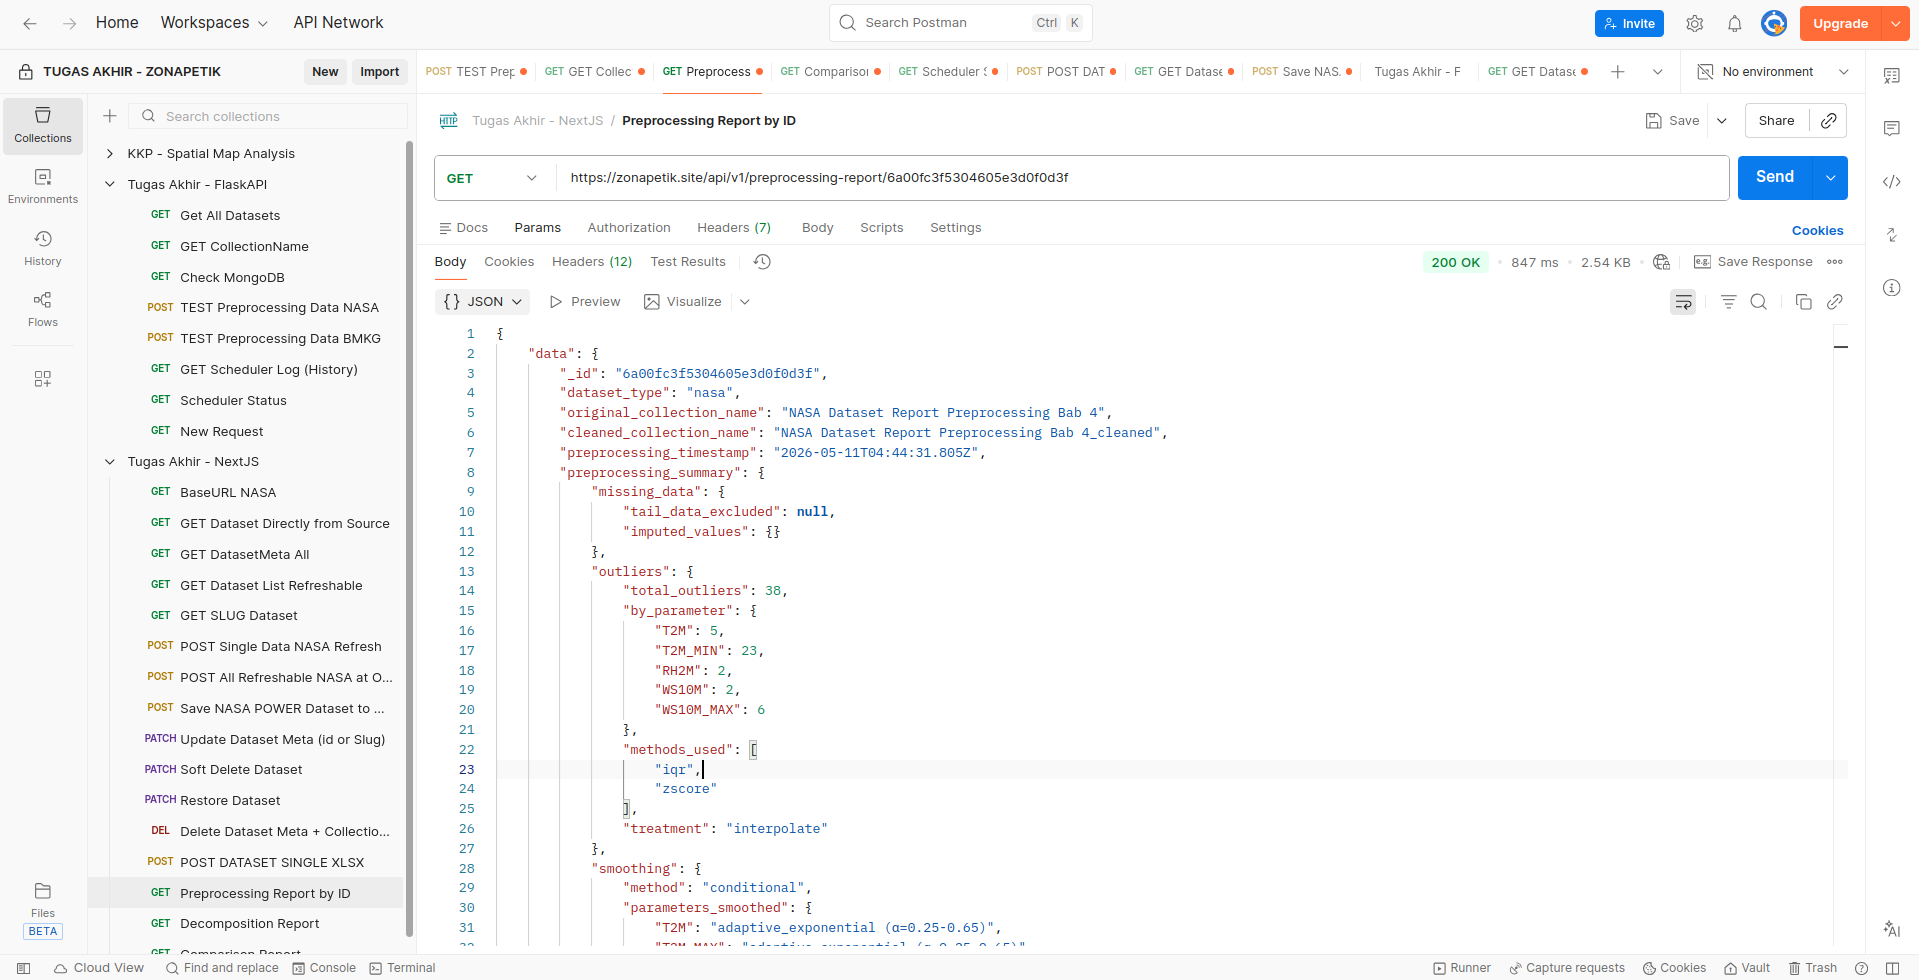
\includegraphics[width=\linewidth]{image/lampiran/5_postman.png}
    \caption{Pengujian endpoint REST API dengan Postman}
    \label{lamp:postman}
\end{figure}
\newpage

% \newappendix{LAMPIRAN 6. BIODATA PENULIS}
% %\includepdf[pages=-]{tanda-tangan/biodata-signed.pdf} --> Jika sudah ada tanda tangan, komen code bawah dan uncomment code ini
% % space kebawah 1 spasi
% \bigskip
% \vspace{1sp}
% % teks dengan font 14 ke tengah
% \begin{center}
%     \fontsize{14}{16}\selectfont
%     \textup{\textbf{BIODATA}}
% \end{center}
% % space kebawah 2 spasi
% \vspace{2sp}

% {\renewcommand{\arraystretch}{1.0}
% \begin{tabular}{@{} p{4.5cm} p{0.2cm} p{8cm} @{}}
% 1. Nama & : & \penulis \\
% 2. Tempat, tanggal lahir & : & \tempatTglLahir \\
% 3. Alamat & : & \alamatPenulis \\
% 4. Nama Ayah & : & \namaAyah \\
% 5. Pekerjaan Ayah & : & \pekerjaanAyah \\
% 6. Nama Ibu & : & \namaIbu \\
% 7. Pekerjaan Ibu & : & \pekerjaanIbu \\
% 8. Alamat Orang Tua & : & \alamatOrtu \\
% 9. Riwayat Pendidikan & : & \\
% \end{tabular}}

% \begin{table}[H]
% \centering
% \resizebox{\textwidth}{!}{%
% \begin{tabular}{|c|c|c|c|c|}
% \hline
% \multicolumn{1}{|l|}{Jenjang} & \multicolumn{1}{l|}{Nama Sekolah} & \multicolumn{1}{l|}{Bidang Studi} & \multicolumn{1}{l|}{Tempat} & \multicolumn{1}{l|}{Tahun Ijazah} \\ \hline
% SD  & \sekolahDasar     & -   & Banda Aceh & \lulusSD \\ \hline
% SMP & \sekolahMenengahPertama & -   & Banda Aceh & \lulusSMP \\ \hline
% SMA & \sekolahMenengahAtas & IPA & Banda Aceh & \lulusSMA \\ \hline
% \end{tabular}%
% }
% \end{table}

% \begin{tabular}{p{7.5cm}l}
% &Banda Aceh, \tanggalBiodata\\
% &\\
% &\\
% &\multirow{1.5}{7.5cm}{\underline{\penulis}} \\ 
% &NPM. \npm \\
% \end{tabular}